% Note to reader: lines beginning with the '%' character are
% 'comments' to you, the human reader of this code, and are 
% ignored by the LaTeX compiler.

%%%%%%%%%%%%%%%%%%%%%%%%%%%%%%%%%%%%%%%%%%%%%%%%%%%%%%%%%%%%%%%%%%
% = Sample template for MIT Junior Lab Student Written Summaries =
% Available from 
%    http://web.mit.edu/8.13/www/Samplepaper/sample-paper.tex
%
% Last Updated July 23, 2014
%
% Adapted from the American Physical Societies REVTeK-4.1 Pages
%    at http://publish.aps.org
%
% ADVICE TO STUDENTS: Each time you write a paper, start with this
%    template and save under a new filename.  If convenient, don't
%    erase unneeded lines, just comment them out using the 
%    '%' character at the start of the line.  Often, they
%    will be useful containers for information.
%
% Using pdflatex, images must be either PNG, GIF, JPEG or PDF.
%    Turn EPS (encapsulated postscript) images to PDF using the
%    epstopdf utility on UNIX systems.
%%%%%%%%%%%%%%%%%%%%%%%%%%%%%%%%%%%%%%%%%%%%%%%%%%%%%%%%%%%%%%%%%%

%%%%%%%%%%%%%%%%%%%%%%%%%%%%%%%%%%%%%%%%%%%%%%%%%%%%%%%%%%%%%%%%%%
% = TO COMPILE THIS DOCUMENT =
%
% From the command line, it would go like this --- assuming you are
%    in the directory where the filename.tex source file and the 
%    filename.bib bibliography file are located, and that you have 
%    permission to create and write files in that directory:
%      > pdflatex filename
%      > bibtex filename
%      > pdflatex filname
%      > pdflatex filename
%    Yes, you run the command several times. The earlier runs 
%    create auxilliary files which keep track of references,
%    citations, equation and section numberring, etc. The later
%    runs combine the information in these auxilliary files with
%    your source document to create the finished product.
%
% If you are using a GUI LaTeX editor like TeXWorks, then there
%    is probably a menu bar button for pdfLaTeX and another for
%    BibTeX. Hit them in the order indicated above. There is 
%    probably also a 'TeXify' button, or something similarly named,
%    which runs all the above commands in one shot.     
%%%%%%%%%%%%%%%%%%%%%%%%%%%%%%%%%%%%%%%%%%%%%%%%%%%%%%%%%%%%%%%%%%


%%%%%%%%%%%%%%%%%%%%%%%%%%%%%%%%%%%%%%%%%%%%%%%%%%%%%%%%%%%%%%%%%%
%  = PREAMBLE =
% The preamble of a LaTeX document is the set of commands that precede
% the \begin{document} line.  It contains a \documentclass line
% to load the REVTeK-4.1 macro definitions and various \usepackage
% lines to load other macro packages.
%
% ADVICE TO STUDENTS: This preamble contains a suggested set of
%     class options to generate a ``Junior Lab'' look and feel that
%     facilitate quick review and feedback from one's peers, TAs,
%     and section instructors.  Don't make substantial changes 
%     to the style without first consulting your section 
%     instructor.
%%%%%%%%%%%%%%%%%%%%%%%%%%%%%%%%%%%%%%%%%%%%%%%%%%%%%%%%%%%%%%%%%%

%\documentclass[aps,twocolumn,secnumarabic,balancelastpage,amsmath,amssymb,nofootinbib, floatfix]{revtex4}
\documentclass[aps,twocolumn,secnumarabic,balancelastpage,amsmath,amssymb,nofootinbib,floatfix]{revtex4-1}

%%%%%%%%%%%%%%%%%%%%%%%%%%%%%%%%%%%%%%%%%%%%%%%%%%%%%%%%%%%%%%%%%%%
% N.B.:  Different computers have different packages installed.  
%        To compile this template in the current Athena 
%        environment, REVTeX 4.1 must be used.  To use the older
%        REVTeX 4, switch which documentclass line above is 
%        commented out above. There are ``bad'' distributions of
%        LaTeX for Windows available on the internet which may 
%        cause users to struggle unjustifiably with REVTeX 4.1.
%
%        If you are unable to compile the template at all, you
%        may need to update your LaTeX packages. (Alternatively, if 
%        your LaTeX distribution includes only the older RevTEX 4,
%        then try changing the documentclass line above. In particular,
%        this approach solves a common compilation problem for users of
%        the TeXWorks editor on Windows, which presents erroneously as a
%        error in the bibliography file.) Don't hesitate to speak 
%        with your section instructor or a TA if you're having 
%        issues getting this template to compile.
%%%%%%%%%%%%%%%%%%%%%%%%%%%%%%%%%%%%%%%%%%%%%%%%%%%%%%%%%%%%%%%%%%%

%%%%%%%%%%%%%%%%%%%%%%%%%%%%%%%%%%%%%%%%%%%%%%%%%%%%%%%%%%%%%%%%%%%
% = Explanation of documentclass options =
%
% aps, prl stand for American Physical Society and Physical 
%     Review Letters respectively.
% twocolumn permits two columns, of course.
% nobalancelastpage doesn't attempt to equalize the lengths of 
%     the two columns on the last page  as might be desired in a 
%     journal where articles follow one another closely.
% amsmath and amssymb are necessary for the subequations 
%     environment among others. These functionalities can
%     also be added use the usepackage function described below,
%     but REVTeX conveniently includes them as documentclass
%     options.
% secnumarabic identifies sections by number to aid electronic 
%     review and commentary.
% nofootinbib forces footnotes to occur on the page where they are
%      first referenced and not in the bibliography.
% floatfix attempts to help LaTeX decide where to place ``floats'',
%      like figures and plots, when it gets stuck and can't decide
%      by it's normal algorithm.
% REVTeX 4.1 is a set of macro packages designed to be used with 
%      LaTeX 2e. REVTeX is well-suited for preparing manuscripts 
%      for submission to APS journals.
%
% = Other documentclasses =
%
% The 'revtex4' and 'revtex4-1' documentclasses are somewhat 
%    specialized for making documents in the style of the APS
%    journals. For a more standard or generic looking LaTeX paper,
%    you could try any of the built-in documentclasses, in 
%    particular 'article' or 'report'. Someday, you may try to use 
%    the 'mitthesis'  documentclass available for download from the 
%    MIT Libraries. The vast majority of source code written for 
%    one documentclass should work just fine in any other, but 
%    occasional quirks arise. For example, some documentclasses 
%    disagree on whether the abstract declaration should come 
%    before or after the \begin{document} declaration.
% 
%%%%%%%%%%%%%%%%%%%%%%%%%%%%%%%%%%%%%%%%%%%%%%%%%%%%%%%%%%%%%%%%%%%

%% Now, include some packages which provide new commands that 
%% extend LaTeX's capabilities. Note that the nearly-essential
%% AMS math packages were added already as documentclass options
%% for REVTeX, but could have been added here using 
%% \usepackage{amsmath}, etc. The pacakges below are commonly 
%% useful, but there are many, many more available to solve a 
%% multitude of typesetting quandries (google your problem), 
%% and you  probably have the necesary packages installed on your
%% system already. Among the examples listed below, this sample
%% document only actually makes use of the 'graphicx', 'bm', 
%% and 'hyperref' pacakges, so the others are commented out for
%% tidyness.


\usepackage{graphicx}      % tools for importing graphics
%\usepackage{lgrind}        % convert program code listings to a form 
                            % includable in a LaTeX document
%\usepackage{xcolor}        % produces boxes or entire pages with 
                            % colored backgrounds
%\usepackage{longtable}     % helps with long table options
%\usepackage{epsf}          % old package handles encapsulated postscript issues
\usepackage{bm}            % special bold-math package. usge: \bm{mathsymbol}
%\usepackage{asymptote}     % For typesetting of mathematical illustrations
%\usepackage{thumbpdf}
\usepackage[colorlinks=true]{hyperref}  % this package should be added after 
                                        % all others.
                                        % usage: \url{http://web.mit.edu/8.13}


%%%%%%%%%%%%%%%%%%%%%%%%%%%%%%%%%%%%%%%%%%%%%%%%%%%%%%%%%%%%%%%%%%%
% And now, begin the document...
%%%%%%%%%%%%%%%%%%%%%%%%%%%%%%%%%%%%%%%%%%%%%%%%%%%%%%%%%%%%%%%%%%%

\begin{document}
\title{Writing Scientific Reports for Junior Lab Using \LaTeX}
\author{Fiz A. Cist}
\email{nobody@mit.edu}
\homepage{http://web.mit.edu/8.13/} %If you don't have one, just comment out this line.
\date{\today}
\affiliation{MIT Department of Physics}


\begin{abstract}
This paper is a written summary and template document for use by
 MIT Physics Junior Lab students like you in preparing your 
experimental reports. It uses \LaTeX\ (pronounced \emph{lay-tek} 
or \emph{lah-tek}, but never \emph{lay-teks}) and the REV\TeX\ macro 
package from the American Physical Society to produce a 
professional quality document.  REV\TeX\ is the standard package 
used to prepare most articles in the Physical Review and  
many other journals as well. 
This example template demonstrates several common 
\LaTeX\ ``tricks'', but the extent of the examples may be too much 
for first time \LaTeX\ users. A simpler ``minimal example'' template 
is also available from the Junior Lab web pages.
 In regards to content, the individual summary you hand in should 
show evidence of your own mastery of the entire experiment. It should 
also possess a neat appearance with concise  and correct English.  The abstract 
is essential. It should briefly mention the motivation, the method, and 
most importantly the quantitative result and its uncertainties.  Based on
those elements, readers may drawn their own conclusion.  The 
length of the paper should be no more than two double-sided pages
 including all figures.  With your instructor's advanced permission, 
appendices can be used for additional plots of raw data, but should 
not be used to simply extend turgid prose!
\end{abstract}

\maketitle




%%%%%%%%%%%%%%%%%%%%%%%%%%%%%%%%%%%%%%%%%%%%%%%%%%%%%%%%%%%%%%%%%%

An important part of your education as a physicist is learning to
use standard tools which enable you to share your work with others.
In Junior Lab, you will be instructed in the use of \LaTeX\ on 
either MIT's Athena environment or your own personal computer. You
will learn to write scientific papers in a widely accepted 
professional style. The source file\footnote{\url{http://web.mit.edu/8.13/www/Samplepaper/sample-paper.zip}}
for this document may be used as a template for your Junior Lab
papers. Spending a few hours studying and altering this document
will allow you to develop sufficient mastery of \LaTeX\ to easily
generate all manner of technical documents.  Specific instructions
for compiling \LaTeX\ documents on various operating systems are
contained in the Appendices.  

The writing
process \cite{owc_process}
involves at least four distinct steps: prewriting, drafting,
revising, and editing.  Given the tight time constraints in Junior
Lab, you are advised to begin the drafting process \emph{before}
finishing your lab sessions.  While final results and analysis are
not possible, much of the draft can be accomplished during the
latter sessions of an experiment.

This is the introductory section of the paper. Your introduction should 
\emph{succinctly} report the motivation, purpose, and relevant background
 to the experiment in way that is accessible to your audience. For Junior Lab, 
the appropriate audience is a stereotypical Junior Lab student who has 
background knowledge and experience similar to your own, but is totally 
unfamiliar with your experiment.


%%%%%%%%%%%%%%%%%%%%%%%%%%%%%%%%%%%%%%%%%%%%%%%%%%%%%%%%%%%%%%%%%%%%%%%%%%%%
% This is a basic figure drawn using the asymptote package
% see http://asymptote.sourceforge.net/ for more information
%\begin{figure}
%\centering
%\begin{asy}
%size(3cm);
%draw(unitcircle);
%\end{asy}
%\caption{Embedded Asymptote Figure} \label {fig:asymptote1}
%\end{figure}
%%%%%%%%%%%%%%%%%%%%%%%%%%%%%%%%%%%%%%%%%%%%%%%%%%%%%%%%%%%%%%%%%%%%%%%%%%%%%
\section{Problem and Relevant Theory}

The report should be type-written in a form that would be suitable
for submission as a manuscript for publication in a professional
journal such as Physical Review Letters. One helpful resource is the 
\textit{APS Physical Review Style and Notation Guide} \cite{aps2011}. Another is the \textit{AIP Style Manual} \cite{aip1990}. Figures (created
as PDF or PNG files) should be inserted into the text in their natural
positions. The body of the summary should include a discussion of
the theoretical issues addressed by the experiment. This should be
done at a level such that another 8.13 student could follow your
development.

%\subsection{Expository Writing}
One of the most important resources for developing into a strong
technical writer is the MIT Writing Center \cite{owc}.
Students should thoroughly investigate the resources on this site 
in the first weeks of 8.13.  Note that students can receive free
consultation ---  online or in person --- on their written reports
through this office!

 The essence of expository writing is the communication of understanding
through a clear and concise presentation of predominately factual
material \cite{mayfield1998,pritchard1990}. Most people cannot
compose successful expository prose unless they put the need to
communicate foremost among their priorities. Two things predominate
in generating understanding in the reader:
\begin{description}
\item[Organization] The reader must be provided with an overview or
outline, know how each fact that he reads fits into that overall
picture, and he must be alerted if it is an especially important
fact. Furthermore, the facts must be presented in a logical order, 
so that fact 17 is not important for understanding fact 12.
\item[Uniform depth of presentation] Bearing in mind the 
preexisting knowledge of the reader, the writer must budget the 
length of discussion allotted to each topic in proportion to its 
importance.
\end{description}
Of course clarity of presentation and elegance of explanation will
greatly enhance the ease and pleasure of understanding; still, a
murky explanation can be fairly useful if the reader has been told
what he is reading about and where it fits into the overall scheme
of things --- especially if the reader is familiar with the general
subject matter under discussion.

The Junior Lab write-up is one of the few opportunities
undergraduate physics majors at MIT are given to practice 
technical writing. Thus, you are urged to concentrate on your 
overall presentation, not only on the
facts themselves. We strongly recommend that you:
\begin{enumerate}
\item Base your report on an outline.
\item \label{en:topic} Begin each paragraph with a topic sentence 
which expresses the main area of concern and the main conclusion 
of the paragraph. Put less important material later in the 
paragraph.
\end{enumerate}
Point~\ref{en:topic} is frequently absent in 8.13 reports. Topic 
sentences are your mechanism for telling the reader what the 
topic under discussion is and where it fits into the overall 
picture.
You can check your topic sentences by reading them in order, 
\textit{i.e.}\ omit all the following sentences in each 
paragraph.  This should give a fair synopsis of your paper.

If you are individually writing up results you obtained with a
partner, use ``we'' and ``I'' appropriately. Note the following admonition
from the \textit{AIP Style Manual} \cite[Section III.A.9]{aip1990}:
\begin{quote}
The old taboo against using the first person in formal prose has long been deplored by the best authorities and ignored by some of the best writers. ``We'' may be used naturally by two or more authors in referring to themselves; ``we'' may also be used to refer to a single author and the author's associates. A single author should also use ``we'' in the common construction that politely includes the reader: ``We have already seen\ldots .'' But never use ``we'' as a mere substitute for ``I,'' as in, for example, ``In our opinion\ldots,''which attempts modesty and achieves the reverse; either write ``my'' or resort to a genuinely impersonal construction.
\end{quote}

Use the past tense for your procedure and analysis, the past 
perfect for preparation and the present for emphasis or 
conclusions. For example, 
``Since we had previously measured constructive and destructive
interference, we concluded that electrons are waves.''

Some further tips:
\begin{itemize}
\item Be sure your figures have comprehensible captions.
\item Make a complete estimate of your errors  --- not just 
statistical --- even if it is crude.
\item Trace the origin of formulae you use 
(\textit{e.g.}\ Moseley's law) to well known physics (in this 
case, to the Bohr atom).  Do \emph{not} derive: just indicate what new 
assumptions are needed.
\end{itemize}

Please consult the MIT Writing and Communications Center's
web page \cite{owc} for further guidance in all aspects of
writing, style, and to make appointments with consultants for free
advice.  They even have an online tutor to which you can submit
sections of your paper for critique at any stage of the writing
process!

Lastly: Remember to \emph{proofread your paper for spelling and grammar
 mistakes}.  Few things are as offensive to a reviewer as careless
 writing. Such mistakes will count against you!

%%%%%%%%%%%%%%%%%%%%%%%%%%%%%%%%%%%%%%%%%%%%%%%%%%%%%%%%%%%%%%%%%%%%%%%%%%%%%
\section{Experimental Sketch and Salient Details}

Here is an example first sentence of an experimental section:
The experimental apparatus consists of a specially prepared chemical
sample containing $^{13}$CHCl$_3$, an NMR spectrometer, and a control
computer, as shown in Fig.~\ref{fig:samplefig}.
%
% Note, when including figures in a \TeX\ document,
% we suggest you first create the figures as
% PDF files and then include them in the following way ,
% without the \texttt{.pdf} suffix)
%
\begin{figure*}[htb]
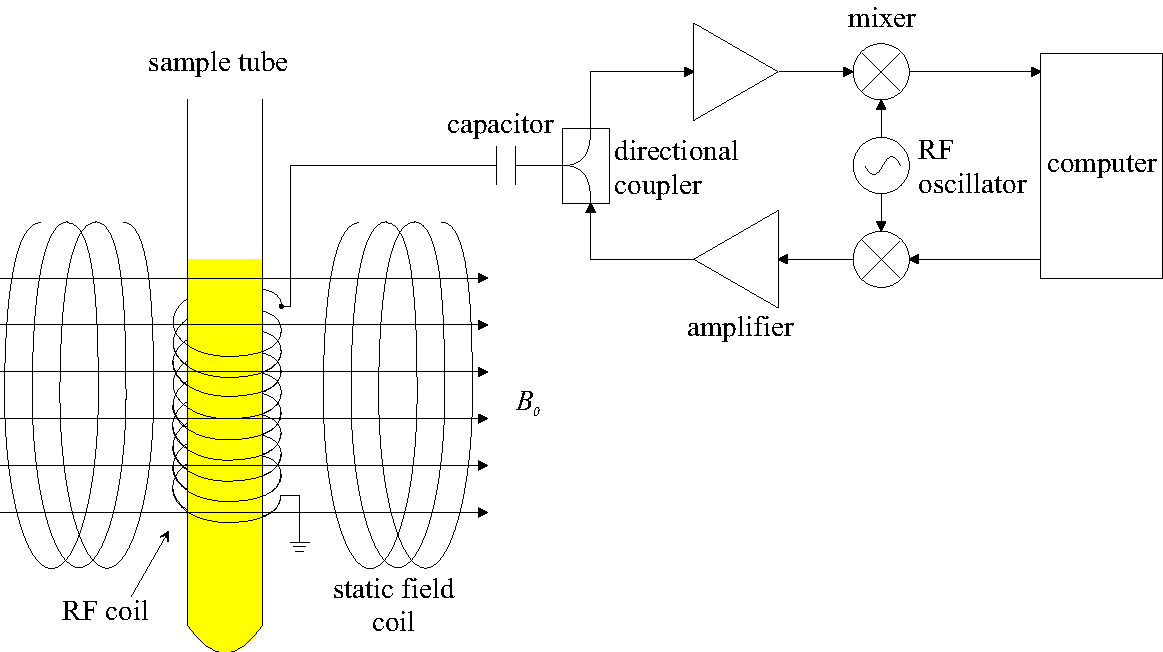
\includegraphics[width=\textwidth]{sample-fig1}
\caption{This is a schematic of the main apparatus.  Use the caption
space to elaborate on specific issues, complications, or operating
procedures.  This is especially valuable given the limited amount of space in
the main body of text.  The size of this graphic was set by the \texttt{width}
command option. The aspect ratio defaults to 1.0 if the height is not also
set. Note, this figure spans two columns, instead of just one. This effect was 
accomplished using the \texttt{figure*} environment instead of just 
\texttt{figure}. Use this effect \emph{sparingly}: single-column figures should suffice in most circumstances. Adapted from \cite{melissinos1966,melissinos2003}.
\label{fig:samplefig}}
\end{figure*}

This section describes the main components of the apparatus and
procedures used. It always makes reference to a figure(s) which
contains a block diagram or schematic of the apparatus and perhaps
includes the most important signal processing steps. The figure
should be referenced as early as possible in this section with the
placement of the figure as close to the descriptive text as is
possible.  It is usually necessary to place additional information
within the figures themselves or in their captions for which there is
no room in the main body of text.  This will help you stay within the
four page limit.


\subsection{Typesetting Mathematics}

One of the great powers of \LaTeX\ is its ability to typeset all
manner of mathematical expressions.  While it does take a short
while to get used to the syntax, it will soon become second nature.
Numbered, single-line equations are the most common type of equation
in Junior Lab papers. For example,
\begin{equation}
   \chi_+(p)\lesssim \left[2 |\bm{p}| (|\bm{p}|+p_z) \right]^{-1/2}
   \left(
   \begin{array}{c}
      |\bm{p}|+p_z\\
      px+ip_y
   \end{array} \right) . \label{eq:first-equation}
\end{equation}
 Be sure there is \emph{no empty line} in your \LaTeX\ source code between
 \verb+\end{equation}+ and the following body text unless you  want 
a new paragraph to start there (and be indented). Also, remember to punctuate 
your equations according to their usage as parts of sentences.

Mathematics can also be placed directly in the text using
\verb+$+ deliminators: the energy $E$ is related to the mass $m$ via $E=mc^2$,
 where $c$ is the speed of light. As in the previous sentence, you should use 
this construction not just for whole equations in running text, but also for 
referring to individual variables by name: otherwise the variables will be set 
in different typefaces when appearing in text versus equations.

Infrequently, you may wish to typeset long equations which span more
than one line of a two-column page.  A good solution is to split up
the equation into multiple lines and label all lines with a single
equation number, as in Equation~\eqref{eq:multilineeq}.  See the
\LaTeX\ source to see how this is done using the \texttt{multline} environment.
%
\begin{multline}
  \sum \vert M^{\text{viol}}_g \vert ^2
   =  g^{2n-4}_S(Q^2)~N^{n-2} (N^2-1) \\
     \times \left( \sum_{i<j}\right) \sum_{\text{perm}}
            \frac{1}{S_{12}}  \frac{1}{S_{12}} \sum_\tau c^f_\tau  \label{eq:multilineeq}.
\end{multline}
%
Since \LaTeX\ does not know mathematical grammar, you have to tell it the appropriate place to split the input using the \verb+\\+ sequence. Here is an example of not simply splitting a long equation across lines, but also having multiple equations for which the equality signs should align on the page. It uses the \texttt{align} environment:
\begin{align}
\begin{split}
\vec{\psi_1} &= |\psi_1\rangle\\ 
         &\equiv c_0|0\rangle + c_1|1\rangle \chi^2\\
        &\approx \prod\sum\left[\frac{y_i-f(x_i)}{\sigma_i}\right]^2 
                    |\psi_1\rangle 
\end{split} \label{eq:split}\\
         Q(z)  &\sim \lim_{\mu \rightarrow \infty}p(x;\mu) \geq 
                   \frac{1}{\sqrt{2 \pi \mu}} e^{-(x-\mu)^2 / 2\mu}P(x) \\
         \alpha(\delta)   &\ll \int_{-\infty}^x p(x')dx'a \times b \pm c \\
\aleph    &\Rightarrow \nabla \hbar \label{eq:aligneq}.
\end{align}

There are in fact several useful environments\footnote{For example, 
Equation~\eqref{eq:split} gathers several typeset lines as one logical 
equation using the \texttt{split} environment inside the \texttt{align} 
environment.} for splitting equations across multiple lines, but if you 
do not want to memorize them all, then just use the \texttt{align} 
environment. You may encounter older \LaTeX\ code which instead uses the
 \texttt{eqnarray} environment for this purpose. Use of the \texttt{eqnarray}
 environment is deprecated and should be avoided.

Finally, it is often useful to group related equations to denote their
relationship, \textit{e.g.}\ in a derivation.  Enclosing single line and
multiline equations in \verb+\begin{subequations}+ and
\verb+\end{subequations}+ will produce a set of equations that are
``numbered'' with letters, as shown in Equations~\eqref{subeq:1} and
\eqref{subeq:2} below:
\begin{subequations}
\label{eq:whole}
\begin{equation}
f(u)^n=  \left\{
      abc123def+\alpha\beta\gamma\delta-1234556\alpha\beta
       \frac{1\sum^{a}_{b}}{A^2}
  \right\}/42 ,\label{subeq:1}
\end{equation}
\begin{multline}
  {\cal M} = ig_Z^2(4E_1E_2)^{1/2}(l_i^2)^{-1}
                (g_{\sigma_2}^e)^2\chi_{-\sigma_2}(p_2) \\
  \times [\epsilon_i]_{\sigma_1}\chi_{\sigma_1}(p_1).\label{subeq:2}
\end{multline}
\end{subequations}

\subsection{Plagiarism: Don't Do It}
It is worth mentioning here some thoughts on ethics and writing
in science.

When you read the report of a physics experiment in a reputable
journal (\textit{e.g.}\ Physical Review Letters) you can generally assume it
represents an honest effort by the authors to describe exactly what
they observed. You may doubt the interpretation or the theory they
create to explain the results. But at least you trust that if you
repeat the manipulations as described, you will get essentially the
same experimental results.

Nature is the ultimate enforcer of truth in science. If subsequent
work proves a published measurement is wrong by substantially more
than the estimated error limits, a reputation shrinks. If fraud is
discovered, a career may be ruined. So most professional scientists
are very careful about the records they maintain and the results and
errors they publish.

In keeping with the spirit of trust in science, Junior Lab instructors
will assume that what you record in your lab book and report in your
written and oral presentations is exactly what you have observed.

\textbf{Fabrication or falsification of data, using the results of
another person's work without acknowledgement, or copying from the 
internet or ``\emph{living group bibles}'' are intellectual crimes 
as serious as plagiarism, and possible causes for dismissal from 
the Institute.}

The acknowledgement of other people's data also applies to the use
of other people's rhetoric. The appropriate way to incorporate an
idea which you have learned from a textbook or other reference is to
study the point until you understand it and then put the text aside
and state the idea in your own words.

One often sees, in a scientific journal, phrases such as ``Following
Bevington and Melissinos \cite{bevington2003, melissinos1966} \ldots''
This means that the author is following the ideas or logic of these
authors and not their exact words.

If you do choose to quote material, it is not sufficient just to
include the original source among the list of references at the end of
your paper. If a few sentences or more are imported from another
source, that section should be
\begin{quote}indented on both sides or enclosed in
quotes, and attribution must be given immediately in the form of a
reference note. \cite{melissinos1966}
\end{quote}

If you have any question at all about attribution of sources, please
see your section instructor.
Further information about how to avoid plagiarism is available
from the MIT Writing Center at 	
\url{http://goo.gl/7PwXJe}.
%\url{http://cmsw.mit.edu/writing-and-communication-center/avoiding-plagiarism/}.





%%%%%%%%%%%%%%%%%%%%%%%%%%%%%%%%%%%%%%%%%%%%%%%%%%%%%%%%%%%%%%%%%%%%%%%%%%%%%
\section{Data Presentation and Error Analysis}


Graphics, such as Fig.~\ref{fig:calibration}, should be well
thought out and crafted to maximize their information content while
retaining clarity of expression.  

\begin{figure}[htb]
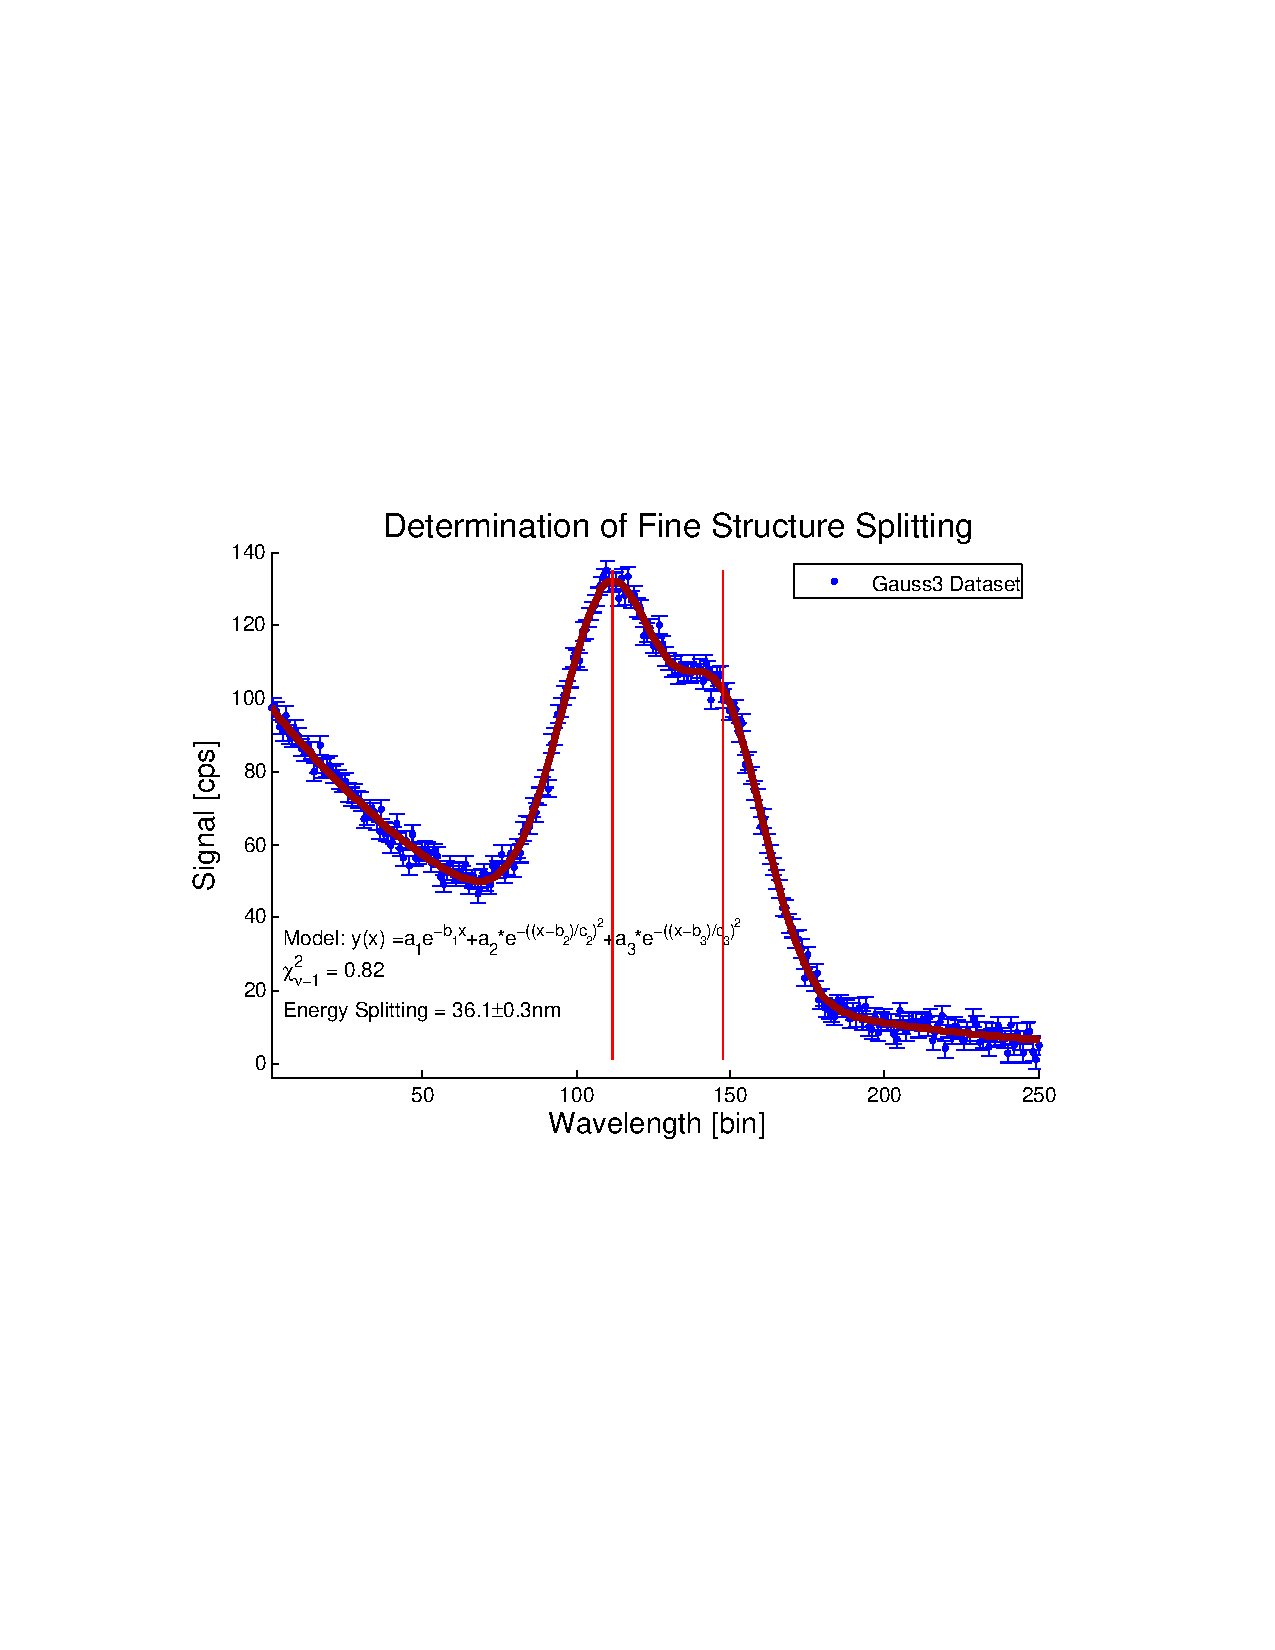
\includegraphics[width=9cm]{sample-fig2.pdf}
\caption{Sample figure describing a set of data, fit procedures and
results, created using the Junior Lab \textsc{Matlab} template script at
\url{http://web.mit.edu/8.13/matlab/fittemplate11.m}. Use the caption space to provide more details about the
fitting procedure, results, or implications if you do not have
sufficient room in the main body of text.}
\label{fig:calibration}
\end{figure}

All papers should have at least one graphic showing an assemblage
of raw data, sometimes placed as an appendix as in
Fig.~\ref{fig:landscapegraphic}. Often these primary data are
analyzed in a specific way that needs to be clearly communicated to
the reader.  In many physics experiments, the peak positions in an
energy spectrum may be required. A graphic demonstrating a typical
fit result, functional model, and reduced $\chi^2$ is shown in
Fig.~\ref{fig:calibration}. Finally, there should be one graphic
which summarizes the experimental data, and which conveys the primary
finding(s) of the laboratory exercise (\textit{e.g.}\ the Geiger-Nuttall
relationship in Fig.~\ref{fig:frenchtaylor}, Moseley's law, the
rotation curve of the Milky Way, the Compton scattering energies \textit{vs.}\
angle, \textit{etc.}). You may find that you need more, but these three should
be a minimum. Finally, it can be useful in \emph{some} circumstances to
have a table of results, see Table~\ref{tab:table1}.

If you reuse graphics from your
paper in oral presentation slides, make sure to increase the size of
all the fonts so that they remain legible from 20 feet away!

%\begin{figure*}[htb]
%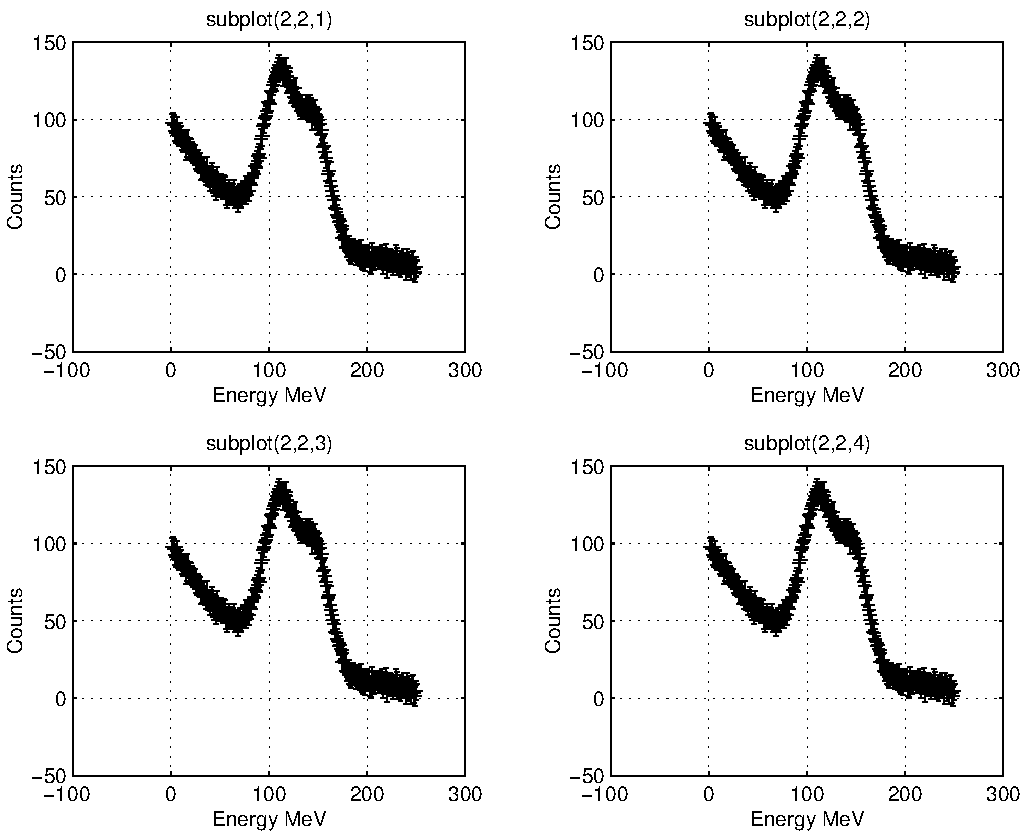
\includegraphics[angle=0,width=10cm]{sample-fig3}
%\caption{Sample paneled figure created in \textsc{Matlab} using the
%\texttt{subplot(2,2,x)} command where \texttt{x} is the element of the plot array into
%which all subsequent commands such as \texttt{plot(x,y)} and \texttt{xlabel('Volts')},
%\textit{etc.}\ get processed.  Use the caption space to provide more details
%about the data, their acquisition or how they were processed if you do
%not have sufficient room in the main body of text.  Figures can be
%rotated using the angle command, see the \TeX\ file for details.  If a
%figure is to be placed after the main text use the ``\texttt{figure*}'' option
%to make it extend over two columns, see the \LaTeX\ file for how this
%was done.}
%\label{fig:panel2x2}
%end{figure*}

\begin{figure}[htb]
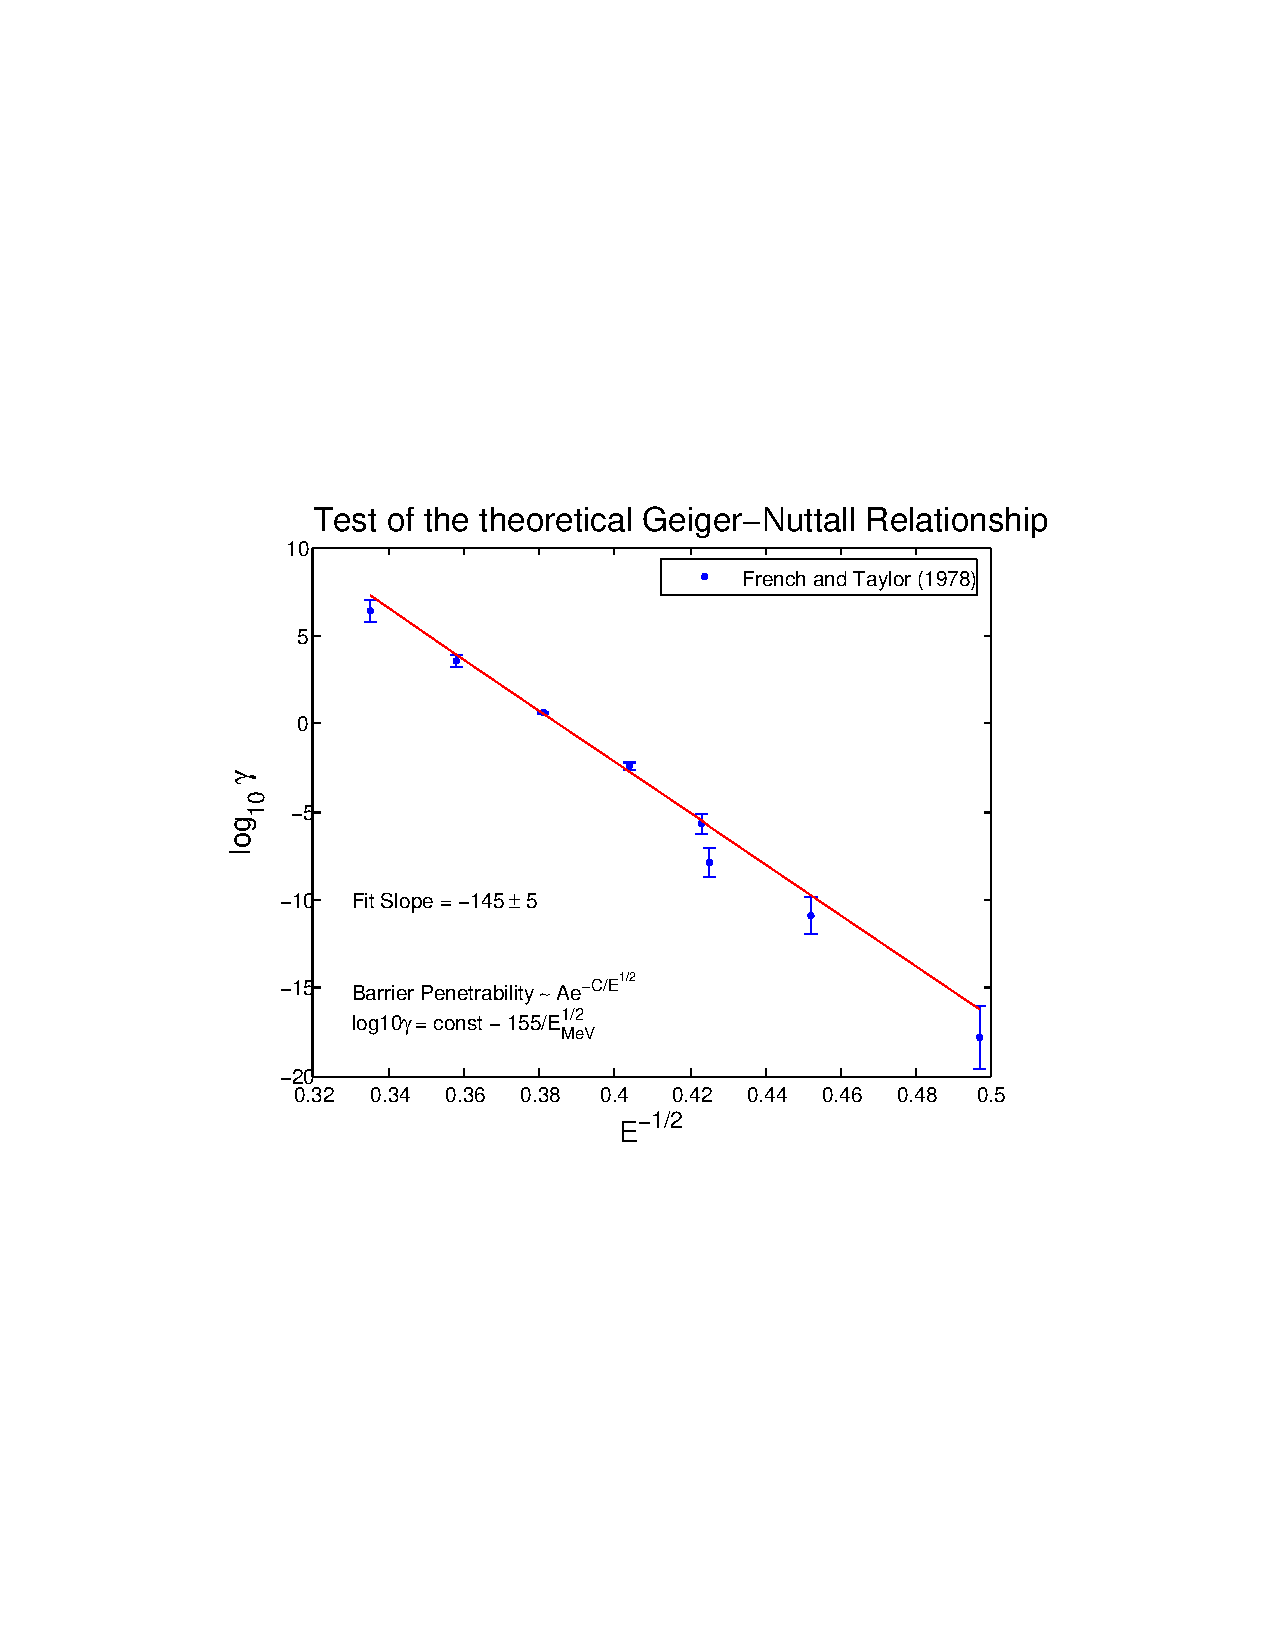
\includegraphics[width=9cm]{frenchtaylor.pdf}
\caption{Sample figure showing overall physical relationship you set
out to test, created using the same script as Fig.~\ref{fig:calibration}.
%\url{http://web.mit.edu/8.13/matlab/fittemplate11.m}
}
\label{fig:frenchtaylor}
\end{figure}

Try to avoid the temptation to inundate the reader with too many
graphics.  It is worth spending some time thinking of how best to
present information rather than just creating graph after graph of
uninformative data.  All figures and tables must be properly
captioned.  As always, material and ideas drawn from the work of others must be
properly cited.

\begin{table}[h]
\caption{\label{tab:table1}An example table with footnotes.  Note
that several entries share the same footnote. Always use a preceding
zero in the data you record in tables.  \emph{Always display units}!
 Inspect the \LaTeX\ source for this table to see exactly how it is
done.}
\begin{ruledtabular}
\begin{tabular}{cccccccc}
 &$r_c$ (\AA) &$r_0$ (\AA)&$\kappa r_0$&
 &$r_c$ (\AA) &$r_0$ (\AA)&$\kappa r_0$\\
\hline
Cu& 0.800 & 14.10 & 2.550 &Sn\footnotemark[1] & 0.680 & 1.870 & 3.700 \\
Ag& 0.990 & 15.90 & 2.710 &Pb\footnotemark[1] & 0.450 & 1.930 & 3.760 \\
Tl& 0.480 & 18.90 & 3.550 & & & & \\
\end{tabular}
\end{ruledtabular}
\footnotetext[1]{Here is the first footnote mark, from Ref.~\cite{bevington2003}.}
\end{table}

If circumstances in an experiment are such that you cannot get your
own data (\textit{e.g.}\ broken equipment, bad weather), you may use another 
students' data \emph{provided you acknowledge it \emph{and} have received 
your instructor's explicit permission}.


%%%%%%%%%%%%%%%%%%%%%%%%%%%%%%%%%%%%%%%%%%%%%%%%%%%%%%%%%%%%%%%%%%%%%%%%%%%%%
\section{Conclusions}

The conclusion section is \emph{not} simply a summary of your measurement 
results, but rather a commentary on the scientific meaning of those results.
 Remember to report your results with
appropriate significant digits, units, and uncertainties, \textit{e.g.}\ 
$Q = (2.12 \pm 0.06)$~kg$\cdot$s$^{-1}$.  It is often useful
to express the quality of your result by measuring how many standard
deviations it lies from expected values. 
Do \emph{not} apologize or make 
excuses for your data.% for the quality of your results in the conclusion.

Bibliographies are very important in Junior Lab papers, so some remarks 
are in order.  Beyond the
requisite citation of source material, they provide evidence of your
investigations beyond the narrow scope of the lab manual, something
explicitly required of all Junior Lab students!  Good bibliographies
are doubly important in the real world where they are very (often
the most) important sources of information for researchers entering
the field.  Bibliographic entries are made within a separate \texttt{.bib}
file which gets attached during process of building a final PDF
document.  See this document's \texttt{sample-paper.bib} file for details
on several types of bibliographic entries and their required and
optional fields.

%%%%%%%%%%%%%%%%%%%%%%%%%%%%%%%%%%%%%%%%%%%%%%%%%%%%%%%%%%%%%%%%%%%%%%%%%%%%%
\begin{acknowledgments} FAC gratefully acknowledges Dr.\ Francine Brown for
her early reviews of this manuscript.
\end{acknowledgments}

%%%%%%%%%%%%%%%%%%%%%%%%%%%%%%%%%%%%%%%%%%%%%%%%%%%%%%%%%%%%%%%%%%%%%%%%%%%%%
% Place all of the references you used to write this paper in a file
% with the same name as following the \bibliography command
%%%%%%%%%%%%%%%%%%%%%%%%%%%%%%%%%%%%%%%%%%%%%%%%%%%%%%%%%%%%%%%%%%%%%%%%%%%%%

\bibliography{sample-paper}


%%%%%%%%%%%%%%%%%%%%%%%%%%%%%%%%%%%%%%%%%%%%%%%%%%%%%%%%%%%%%%%%%%%%%%%%%%%%%
\clearpage
\appendix
\section{\LaTeX\ on Windows}
For students who would like to use a Windows platform, \textsc{MiK}\TeX\
(pronounced \emph{mik-tek}) is a freely available implementation of
\TeX\ and related programs available from \url{www.miktex.org}. Note
that \textsc{MiK}\TeX\ itself runs from a command line prompt and is not terribly
convenient unless you are comfortable with the Windows shell.  
%We recommend that you simultaneously 
%install a nice \TeX\ editor/shell such as  \textsc{WinEdt} (available from
%\url{www.winedt.com} for only \$40 for students) or \TeX\textsc{works} 
%(available for free from \url{www.tug.org/texworks} for Windows, MacOS, 
%and Linux). 
Luckily, \textsc{MiK}\TeX\ comes packaged with the \TeX\textsc{works} 
editting environment as a front end to \LaTeX. Many beginners find 
\TeX\textsc{works} easier and more 
intuitive to use than the alternative of a generic text editor and 
command line compliation. Advanced users may prefer a more powerful 
editor like \textsc{Emacs} or \textsc{vi} instead of a \LaTeX-specific
editor like \TeX\textsc{works}.

Note that due to some ``bad'' distributions of \LaTeX\ floating around the 
internet, some Windows users may need to update their \LaTeX\ installation to 
the latest version of REV\TeX-4.1 and the required \texttt{natbib} package. 
Alternatively, they can use the older REV\TeX-4 by changing the
 \verb+\documentclass+ declaration at the beginning of the source file. 
You will know if you need to do this if you attempt to compile this sample 
document and receive errors about bad bibliography entries.

Once you have installed the above software, you will need to download
the source files listed in the next section and put them on your
Windows machine in order to ``rebuild'' this document from scratch.

%If you wish to view postscript files under Windows, we
%suggest downloading and installing \textsc{Ghostscript} available from
%\url{www.cs.wisc.edu/~ghost}.

\section{\LaTeX\ on Athena}
For students wishing to utilize MIT's Athena environment, the
 process to create your documents is quite simple.  You can use the following
commands verbatim or tweak them to suit your own organizational system.

In your home directory on Athena, create a convenient directory structure 
for all of your Junior Lab
work by typing:
\begin{verbatim}
> mkdir ~/8.13
> mkdir ~/8.13/papers
> mkdir ~/8.13/papers/template
> cd ~/8.13/papers/template
\end{verbatim}
Once this (or similar) directory structure has been created, copy all
of the files needed to compile the template from the Junior Lab locker
into your own Athena account by typing:
%> setup 8.13
\begin{verbatim}
> cp /mit/8.13/www/Samplepaper/sample-zipped/* .
\end{verbatim}
The final period above places the
copied files into the current directory so make sure you are in the
correct directory!
%The \texttt{setup} command automatically
%appends to your path the location of the REV\TeX-4.1 files.
  You can see where you are by typing:
\begin{verbatim}
> pwd
\end{verbatim}
The following files should now be in
your current directory:
\begin{verbatim}
sample-paper.tex
sample-paper.bib
sample-paper.pdf
sample-fig1.pdf
sample-fig2.pdf
sample-fig3.pdf
typical-fit-plot.pdf
frenchtaylor.pdf
lgrind.sty
\end{verbatim}
Additional files may also have been copied but do not worry: these get
regenerated when you build your PDF document.

Now build the file (omitting the \texttt{.tex} suffix in the 
following steps):
\begin{verbatim}
> pdflatex sample-paper
> bibtex sample-paper
> pdflatex sample-paper
> pdflatex sample-paper
\end{verbatim}


The repeated calls to \texttt{pdflatex} are necessary to resolve any nested
references in the final PDF file.  The \texttt{bibtex} call reads in the
bibliography file \texttt{sample-paper.bib} allowing citation references to
be resolved.

\textbf{Remember to ``\texttt{ispell -t filename.tex}'' to perform a \LaTeX -safe spell check before handing in your paper!}

\section{Graphics Utilities}
%\subsection{Drawing Programs}

Students should become proficient with a simple vector based
drawing program such as \textsc{inkscape}.
%, \textsc{xfig}, or \textsc{tgif} on Athena.
Every written summary should include one or two simple schematics,
based on your initial hand sketches from your lab notebook

%\subsection{Image Conversion}

It is easy to  convert images from one format to another, \textit{e.g.}\ a
scanned JPEG or bitmap image into a PDF file for inclusion into a
written summary.  A useful utility, available on some Unix machines,  is
\textsc{imconvert}. Typing \texttt{imconvert} without any arguments will show
you the accepted file types.  
%For example, to convert a JPEG image
% to PDF, one types: \\\texttt{> imconvert jpg:filename.jpg pdf:filename.pdf}\\
Other useful conversion utilities include \textsc{ps2pdf}, \textsc{eps2pdf}, and a variety of similar programs.

%\subsection{\textsc{Matlab} and \LaTeX}
\textsc{Matlab} is perhaps the most common tool used by Junior Lab students
for data analysis and representation.  \textsc{Matlab} figures can
incorporate \LaTeX\ symbols in their titles, axes labels, and text
labels.  Figures can be saved directly into PDF or PNG 
format, obviating the need for any further format conversion.

% Surround figure environment with turnpage environment for landscape 
% presentation. The turnpage environment is provided by the revtex 
% documentclass.
\begin{turnpage}
\begin{figure*}[htb]
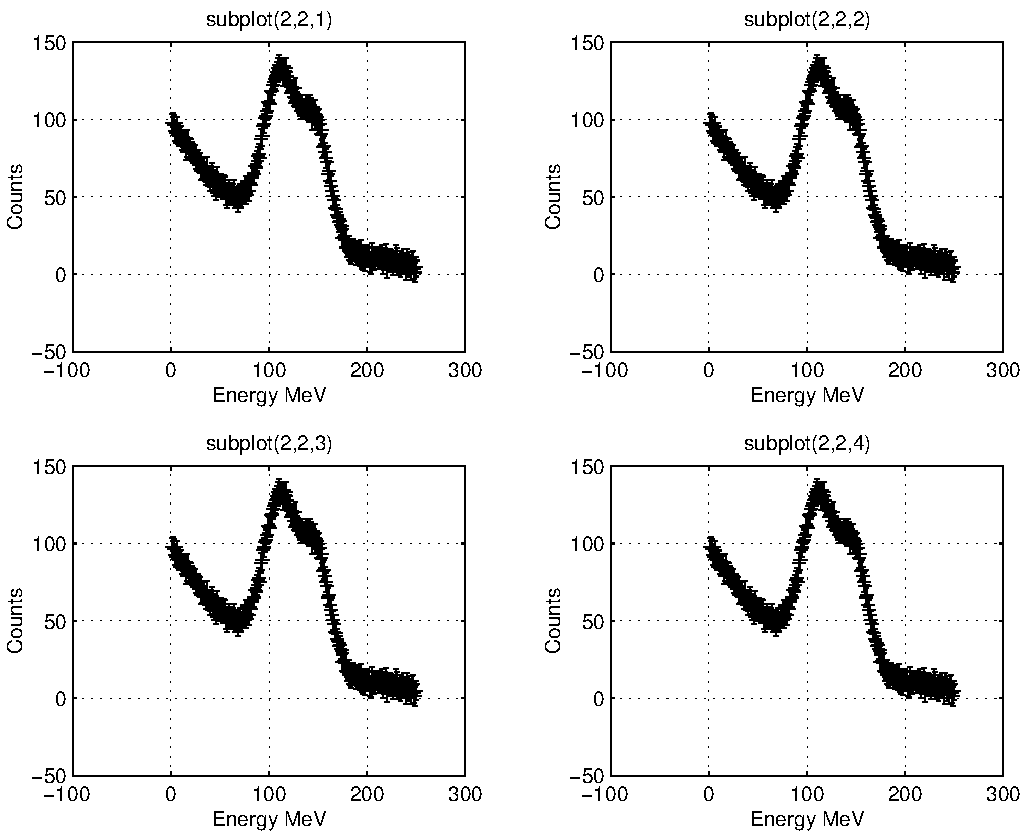
\includegraphics[height=0.89\textwidth]{sample-fig3}
\caption{For very large plots where important detail might be lost
if too compressed, it may be convenient to use the \texttt{turnpage}
environment for displaying in landscape mode, \textit{e.g.}\ any experiment
where a data set is acquired at several angular positions (21~cm,
$e/m$, Rutherford), or is time varying (alpha decay or
pulsed NMR).  These full page graphics are usually best kept in
appendices so as not to impede the flow of the paper.  Note that
large tables can also be presented in this landscape environment if
desired \label{fig:landscapegraphic}}
\end{figure*}
\end{turnpage}

% tables should appear as floats within the text
%
% Here is an example of the general form of a table:
% Fill in the caption in the braces of the \caption{} command. Put the label
% that you will use with \ref{} command in the braces of the \label{} command.
% Insert the column specifiers (l, r, c, d, etc.) in the empty braces of the
% \begin{tabular}{} command.
% The ruledtabular enviroment adds doubled rules to table and sets a
% reasonable default table settings.
% Use the table* environment to get a full-width table in two-column
% Add \usepackage{longtable} and the longtable (or longtable*}
% environment for nicely formatted long tables. Or use the the [H]
% placement option to break a long table (with less control than
% in longtable).
% \begin{table}%[H] add [H] placement to break table across pages
% \caption{\label{}}
% \begin{ruledtabular}
% \begin{tabular}{}
% Lines of table here ending with \\
% \end{tabular}
% \end{ruledtabular}
% \end{table}

% To convert program (e.g. C++ Fortran, Matlab, LaTeX) listings to a
% form easily includable in a LaTeX document
%
% type lgrind -s to see options
% lgrind -llatex -i sample-paper.tex > sampleinputtex
% creates a file sampleinput.tex which can then be included into this
% document simply by uncommenting the next line
%\lgrindfile{testinput.tex}

\end{document}
